\section{Chapter 3: Stellar Energy and Fusion}

\subsection{Where does the energy in stars come from, and how was it conjectured?}
\solutionblock{Was conjectured by Sir Arthur Eddington in 1920s. He realized that the sun gains energy from the mass defect of Hydrogen to Helium.\\ If the sun was a lump of coal it would burn out in a few thousand years.\\ The sun must be older than the earth they argued and the earth is (according to Lord Kelvin) at least 20 million years old [Spoiler: he was was way off].\\}

\subsection{Write the reaction of the proton-proton cycle. Why is it important for stars?}
\solutionblock{
    1) Two protons combine to form deuterium (D) and a positron (e+) and a neutrino ($\nu$)\\
    2) The deuterium combines with another proton to form Helium-3 (He-3) and a gamma ray ($\gamma$)\\
    3) Two Helium-3 nuclei combine to form Helium-4 (He-4) and two protons.\\
    This process releases about 10 million times more energy than the chemical bonding of Hydrogen with Oxygen to form Water. $\rightarrow$ from that we conclude that the sun must live not for thousands, but for billions of years. \\
    \begin{figure}[H]
        \centering
        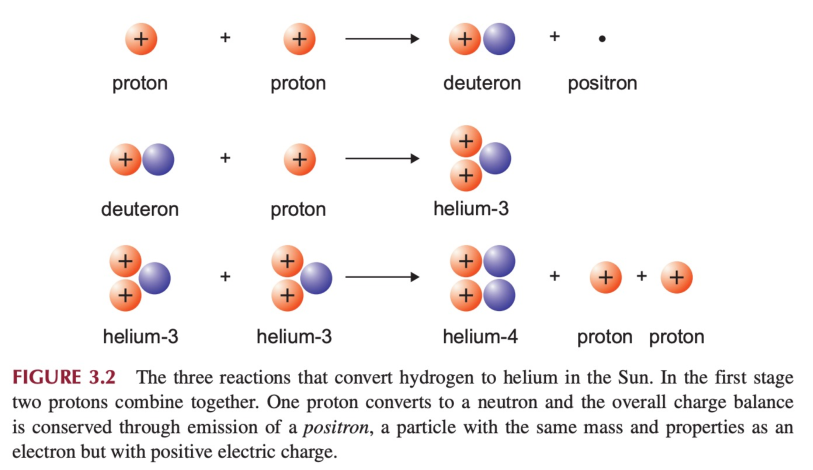
\includegraphics[width=0.8\textwidth]{chapters/fig/3_pp_cycle.png}
        \caption{Proton-Proton Cycle}
        \label{fig:proton_proton_cycle}
    \end{figure}
}

\subsection{How are stars able to generate conditions for fusion, and why do we need other ways on earth?}
\solutionblock{They are massive, so gravity compresses them and heats them up. They have to constantly balance the gravitational force with the pressure from the fusion reaction.\\
In the sun fusion only happens near the core - practically within a sphere 1/10 of the sun's radius. About 270 watts are produced per cubic meter in the core which is then transported through radiation and further out through convection.\\
In the core the sun has a temperature of about 14 million Kelvin while on the surface it is only about 6000 Kelvin.\\
On Earth we need other confinement methods because we need much higher energy densities than the sun.\\}

\subsection{What's the meaning of different star stages and their composition? What stage is the Sun and elements can it produce?}
\solutionblock{One might wonder how heavier elements than Helium are produced.\\
For bigger stars (than our sun) the fusion process continues after Helium-4 is produced. The star burns at a higher temperature and fuses Helium-4 to Carbon-12 and Carbon-12 to Oxygen-16, ... and so on Neon-20, Magnesium-24,...\\
Our sun can only produce Helium-4 and is subsequently doomed to cool down and shrink into a white dwarf.\\
Bigger stars explode in a supernova and produce all the heavier elements which are the building blocks for so called secondary stars (like our sun) and planets and \textit{us}.\\}

\subsection{Explain primordial nucleosynthesis and how it led to the current universe.}
\solutionblock{Also known as Big Bang Nucleosynthesis this refers to the production of nuclei other than Hydrogen during the early phases of the universe.\\ The universe was extremely hot and dense a few seconds after the big bang. As it expanded and cooled down the protons and neutrons combined to form Hydrogen, Helium-4 (pp-cycle) and a small amount of Lithium.\\ By pure change certain regions of the universe had a slightly higher density than others. These regions attracted more matter and eventually formed stars.\\}
